%\documentclass[11pt,a4paper]{article}
\documentclass[11pt,a4paper]{scrartcl}
%\documentclass[11pt,a4paper,oneside]{book}
\usepackage[british,UKenglish,USenglish,english,american]{babel}
%\usepackage[a4paper, total={16cm, 23cm}]{geometry}
\usepackage[tmargin = 1.25in,bmargin = 1.25in,lmargin = 0.75in,rmargin = 0.75in]{geometry}
\usepackage{tikz}
\usepackage{graphicx}
\usepackage{pgfplots}
\pgfplotsset{width=12cm,compat=1.9}
\usepackage{setspace}
\usepackage{chemmacros}
\usepackage{chemfig}
%\usepackage{ghsystem}
%\usechemmodule{redox}
%\usepackage{chemnum}
%\usepackage{bohr}
%\usepackage{elements}
%\usepackage{endiagram}
%\usepackage{modiagram}
%\usepackage{chemgreek}
%\usepackage{mhchem}
\usepackage{esint}
\usepackage{tabularray}

\usepackage{makeidx}
\usepackage{epstopdf}

\usepackage{amssymb}
\usepackage{mathrsfs}
%\usepackage{minted}
\usepackage{bm}
\usepackage{amsmath}
\usepackage{enumitem}
\usepackage[english]{varioref}
\usepackage[english]{babel}
\usepackage{lipsum}
\usepackage{fancyhdr}
\pagestyle{fancy} 
\usepackage{float}
\usepackage{empheq}
\usepackage[framemethod=tikz]{mdframed}
\usepackage{epstopdf}
\numberwithin{equation}{section}
\usepackage{eso-pic}
\usepackage{calc}
\usepackage{nccmath}
\usepackage{caption}
\usepackage{subcaption}
\usepackage{gensymb}
\usepackage{amsfonts,amsthm,epsfig,epstopdf,titling,url,array}
\usepackage{siunitx}
\sisetup{input-digits = 0123456789\pi}
\usepackage[symbol]{footmisc}
\usepackage{xcolor}
\usepackage{multicol}
\usepackage{boondox-cal}
\DeclareSIUnit\atm{atm}
\setcounter{secnumdepth}{3}
\setcounter{tocdepth}{3}
\usepackage{booktabs}
\usepackage{blindtext}
\usepackage{changepage}
\usepackage{longtable}

% \usepackage{draftwatermark}
% \SetWatermarkText{DRAFT}
% \SetWatermarkScale{5}

\DeclareSIUnit\atm{atm}

\pagestyle{fancy} 
\fancypagestyle{firstpage}{
	\rhead{
	}
}
\fancyhead[L]{\small\slshape\nouppercase{\leftmark}}
\chead{}
\rhead{ 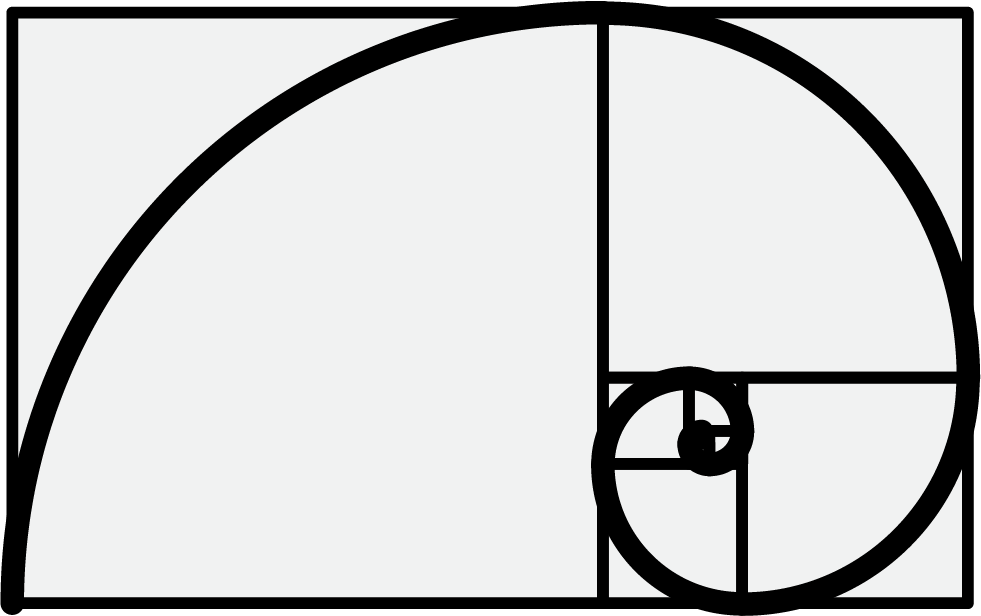
\includegraphics[height=0.75cm]{figures/pwr-control_logo_doc.png}
}
\lfoot{\textit{}}
\cfoot{-\ \thepage\ -}
\rfoot{\textit{}}

\DeclareMathOperator{\rank}{rank}
\DeclareMathOperator{\atantwo}{atan2}
\DeclareMathOperator{\arctantwo}{arctan2}
\DeclareMathOperator{\spn}{span}

\renewcommand{\headrulewidth}{0.4pt}
\renewcommand{\footrulewidth}{0.4pt}
\newcommand{\abs}[1]{\left|#1\right|}
\definecolor{mycolor1}{rgb}{0.97, 0.97, 0.97}
\definecolor{mycolor2}{rgb}{0.97, 0.97, 0.97}
\definecolor{tableShade}{gray}{0.9}
\newcommand{\sign}{\text{sign}}
\newcommand{\centered}[1]{\begin{tabular}{@{}l@{}} #1 \end{tabular}}
\theoremstyle{it}
\newtheorem{defn}{Definition}[section]
\newtheorem{assumption}{Assumption}[section]
\newtheorem{thm}{Theorem}[section]
\newtheorem{lemma}{Lemma}[section]
\newtheorem{corollary}{Corollary}[section]
\theoremstyle{definition}
%\theoremstyle{it}
\newtheorem{example}{Example}[section]
\let\eqrefn\eqref
\renewcommand{\eqref}[1]{Eq.~(\ref{#1})}

\newenvironment{myitemize_1}
{ \begin{itemize}[topsep=4pt]
		\setlength{\topsep}{2pt}		
		\setlength{\itemsep}{2pt}
		\setlength{\parskip}{2pt}
		\setlength{\parsep}{2pt}    }
	{ \end{itemize}                  	}

\newenvironment{myitemize_2}
{ \begin{itemize}[topsep=4pt]
		\setlength{\topsep}{2pt}		
		\setlength{\itemsep}{2pt}
		\setlength{\parskip}{2pt}
		\setlength{\parsep}{2pt}    }
	{ \end{itemize}   					}


\newmdenv[innerlinewidth=0.5pt, roundcorner=4pt,backgroundcolor=mycolor2, 
linecolor=mycolor1,innerleftmargin=6pt,
innerrightmargin=6pt,innertopmargin=6pt,innerbottommargin=6pt]{mybox}

\title{\textbf{ 
		\begin{LARGE}
			Extended Kalman Filter:
		\end{LARGE} \\[24pt]
		\begin{Large}
	Application to IM with Ttype MPC Three Phase Inverter.
	\end{Large}}
}
\author{\textbf{Davide Bagnara}}

\begin{document}
	\thispagestyle{firstpage}
	\begin{mybox}
		\maketitle
		\vspace{125mm}
	\end{mybox}
	\newpage
	\tableofcontents
	\listoffigures	
	\listoftables
	\newpage
	
	{In this document the model of a generic flexible shaft is derived.}

\begin{onehalfspace}
\section{Induction Motor Model Derivation}
In this section we derive the dynamical model of the induction motor for 
control purpose. For the derivation of the dynamical model, the rotor windings 
are assumed to be identical to the stator windings with resistance $R_r$ ($R_s$ 
for the stator winding) and equivalent turns $N_r=N_s$.

Let
\begin{equation} \label{im_eq_1}
	\vec{\psi}^{\,s}_{abc} = \left[\psi_{sa},\,\psi_{sb},\,\psi_{sc}\right]^T 
	\quad\text{stator flux}
\end{equation}
\begin{equation} \label{im_eq_2}
	\vec{\psi}^{\,r}_{abc} = \left[\psi_{ra},\,\psi_{rb},\,\psi_{rc}\right]^T 
	\quad\text{rotor flux}
\end{equation}
be the vectors whose components are the stator and rotor flux linkages, 
respectively, with $a$, $b$, $c$ denoting the three phases components. 
Similarly, let
\begin{equation} \label{im_eq_3}
	\begin{aligned}
		\vec{i}^{\,s}_{abc} = & \left[i_{sa},\,i_{sb},\,i_{sc}\right]^T 
		\quad\text{stator current} \\ 
		\vec{i}^{\,r}_{abc} = & \left[i_{ra},\,i_{rb},\,i_{rc}\right]^T 
		\quad\text{rotor current}
	\end{aligned}
\end{equation}
be the vectors whose components are the stator and rotor currents. Then, for an 
induction motor with one pole pair we can write
\begin{equation} \label{im_eq_4}
	\begin{aligned}
		&\left. \begin{aligned}
			& \frac{d\psi_{sa}}{dt} + R_s i_{sa} = u_{sa} \\[6pt]
			& \frac{d\psi_{sb}}{dt} + R_s i_{sb} = u_{sb} \\[6pt]
			& \frac{d\psi_{sc}}{dt} + R_s i_{sc} = u_{sc} \\[6pt]
		\end{aligned}\right\rbrace \quad\text{respect to the stationary 
			reference frame}\\[6pt]
		&\left. \begin{aligned}
			& \frac{d\psi_{ra}}{dt} + R_r i_{ra} = 0 \\[6pt]
			& \frac{d\psi_{rb}}{dt} + R_r i_{rb} = 0 \\[6pt]
			& \frac{d\psi_{rc}}{dt} + R_r i_{rc} = 0 
		\end{aligned} \right\rbrace \quad\text{respect to the rotor reference 
			frame}
	\end{aligned}
\end{equation}
where the stator and rotor fluxes, under the assumption of linear magnetic 
circuits, satisfy the linear relation
\begin{equation}\label{im_eq_5}
	\begin{aligned}
		\begin{bmatrix} \vec{\psi}^{\,s}_{abc} \\[6pt] \vec{\psi}^{\,r}_{abc} 
		\end{bmatrix} = \begin{bmatrix} \mathbf{L}_s & \mathbf{L}_{m} \\[6pt] 
			\mathbf{L}_{m}^{\,T} & \mathbf{L}_{r} \end{bmatrix}\begin{bmatrix} 
			\vec{i}^{\,s}_{abc} \\[6pt] \vec{i}^{\,r}_{abc} \end{bmatrix}
	\end{aligned}
\end{equation}
where
\begin{equation}\label{im_eq_6}
	\begin{aligned}
		\mathbf{L}_s = \begin{bmatrix} L_\mu+L_s & -\frac{1}{2}L_s & 
			-\frac{1}{2}L_s \\[6pt] -\frac{1}{2}L_s & L_\mu+L_s & 
			-\frac{1}{2}L_s 
			\\[6pt] -\frac{1}{2}L_s & -\frac{1}{2}L_s & L_\mu+L_s \end{bmatrix}
	\end{aligned}
\end{equation}
\begin{equation}\label{im_eq_7}
	\begin{aligned}
		\mathbf{L}_r = \begin{bmatrix} L_\mu+L_r & -\frac{1}{2}L_r & 
			-\frac{1}{2}L_r \\[6pt] -\frac{1}{2}L_r & L_\mu+L_r & 
			-\frac{1}{2}L_r 
			\\[6pt] -\frac{1}{2}L_r & -\frac{1}{2}L_r & L_\mu+L_r \end{bmatrix}
	\end{aligned}
\end{equation}
and
\begin{equation}\label{im_eq_8}
	\begin{aligned}
		\mathbf{L}_m = L_m\begin{bmatrix} \cos(\vartheta_{m}) & 
			\cos(\vartheta_{m}+\frac{2\pi}{3}) & 
			\cos(\vartheta_{m}-\frac{2\pi}{3}) 
			\\[6pt] \cos(\vartheta_{m}-\frac{2\pi}{3}) & \cos(\vartheta_{m}) & 
			\cos(\vartheta_{m}+\frac{2\pi}{3}) \\[6pt] 
			\cos(\vartheta_{m}+\frac{2\pi}{3}) & 
			\cos(\vartheta_{m}-\frac{2\pi}{3}) 
			& \cos(\vartheta_{m}) \end{bmatrix}
	\end{aligned}
\end{equation}
Considering the transformation 
\begin{equation}\label{im_eq_9}
	\begin{aligned}
		& \mathbf{T}_1 = 
		\frac{2}{3}\begin{bmatrix}
			\frac{1}{2} & \frac{1}{2} & \frac{1}{2} \\[6pt]
			1 & -\frac{1}{2} & -\frac{1}{2} \\[6pt]
			0 & \frac{\sqrt{3}}{2} & -\frac{\sqrt{3}}{2} 
		\end{bmatrix}
	\end{aligned} 
\end{equation}
such that 
\begin{equation}\label{im_eq_10}
	\left[
	\begin{matrix}
		i_{s0}		\\
		i_{s\alpha} \\
		i_{s\beta}
	\end{matrix} \right] = \frac{2}{3}\begin{bmatrix}
		\frac{1}{2} & \frac{1}{2} & \frac{1}{2} \\[6pt]
		1 & -\frac{1}{2} & -\frac{1}{2} \\[6pt]
		0 & \frac{\sqrt{3}}{2} & -\frac{\sqrt{3}}{2} 
	\end{bmatrix}
	\left[
	\begin{matrix}
		i_{sa} \\
		i_{sb} \\
		i_{sc}
	\end{matrix} \right]
\end{equation}
in which $\mathbf{T}_1^{-1} = \mathbf{T}_1^T$.
\begin{figure}[H]
	\centering
	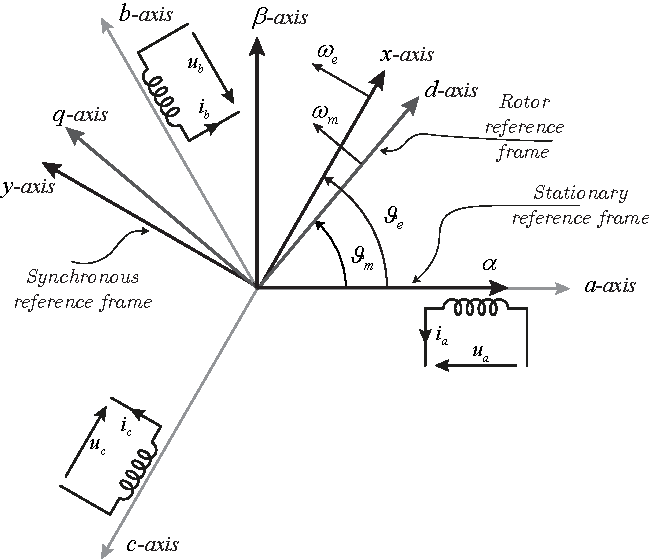
\includegraphics[width = 330pt, 
	keepaspectratio]{figures/kalman/reference_frames_im.pdf}
	\captionsetup{width=.5\textwidth}
	\caption{Machine reference frames description: stationary $(\alpha,\beta)$, 
		rotor $(d,q)$ and synchronous speed $(x,y)$ reference frames.}
	\label{figure_im_ref_frame1} 
\end{figure}
The Eq.~\eqref{im_eq_4} of the induction motor become (considering balanced 
operating conditions, $i_{s0}=0$, $i_{r0}=0$)
\begin{equation}\label{im_eq_11}
	\begin{aligned}
		&\left. \begin{aligned}
			& \frac{d\psi_{s\alpha}}{dt} + R_s i_{s\alpha} = u_{s\alpha} \\[6pt]
			& \frac{d\psi_{s\beta}}{dt} + R_s i_{s\beta} = u_{s\beta} 
		\end{aligned}\right\rbrace \quad\text{stationary reference frame}\\[6pt]
		&\left. \begin{aligned}
			& \frac{d\psi_{rd}}{dt} + R_r i_{rd} = 0 \\[6pt]
			& \frac{d\psi_{rq}}{dt} + R_r i_{rq} = 0 
		\end{aligned}\right\rbrace \quad\text{rotor reference frame}\\[6pt]
		&\left. \begin{aligned}
			& \dot{\vartheta} = \omega_m \\[6pt]
			& J\dot{\omega}_m = \tau_e -\tau_l
		\end{aligned}\right\rbrace \quad\text{mechanical equations}
	\end{aligned}
\end{equation}
where $(\psi_{rd},\, \psi_{rq})$ and  $(i_{rd},\, i_{rq})$ denote the $(d,\,q)$ 
components of the rotor flux and rotor current in the $(d,q)$ reference frame 
attached to the rotor, rotating at rotor speed $\omega_m = \dot{\vartheta}_m$, 
while $(\psi_{s\alpha},\, \psi_{s\beta})$ and  $(u_{s\alpha},\, u_{s\beta})$ 
denote the components of the stator flux and the stator voltage vectors in the 
fixed reference frame.

The linear operator for changing of coordinates between stationary reference 
frame and rotor reference frame is
\begin{equation}\label{im_eq_12}
	\mathbf{T}_2(\vartheta_{m})=\begin{bmatrix}
		\cos\vartheta_m & \sin\vartheta_m \\[6pt]
		-\sin\vartheta_m & \cos\vartheta_m
	\end{bmatrix} \qquad
	\mathbf{T}_2^{-1}(\vartheta_{m})=\begin{bmatrix}
		\cos\vartheta_m & -\sin\vartheta_m \\[6pt]
		\sin\vartheta_m & \cos\vartheta_m
	\end{bmatrix}
\end{equation}
such that
\begin{equation}\label{im_eq_13}
	\left[
	\begin{matrix}
		i_{rd} \\
		i_{rq}
	\end{matrix} \right] = 
	\left[
	\begin{matrix}
		\cos\vartheta_m & \sin\vartheta_m \\[6pt]
		-\sin\vartheta_m & \cos\vartheta_m
	\end{matrix} \right]
	\left[
	\begin{matrix}
		i_{r\alpha} \\[6pt]
		i_{r\beta}
	\end{matrix} \right]
\end{equation}
\begin{equation}\label{im_eq_14}
	\left[
	\begin{matrix}
		\psi_{rd} \\[6pt]
		\psi_{rq}
	\end{matrix} \right] = 
	\left[
	\begin{matrix}
		\cos\vartheta_m & \sin\vartheta_m \\[6pt]
		-\sin\vartheta_m & \cos\vartheta_m
	\end{matrix} \right]
	\left[
	\begin{matrix}
		\psi_{r\alpha} \\[6pt]
		\psi_{r\beta}
	\end{matrix} \right]
\end{equation}
with $(\psi_{r\alpha},\psi_{r\beta})$ and $(i_{r\alpha}, i_{r\beta})$ denoting 
the $(\alpha,\beta)$-components of the rotor flux and current in the fixed 
frame.
\begin{figure}[H]
	\centering
	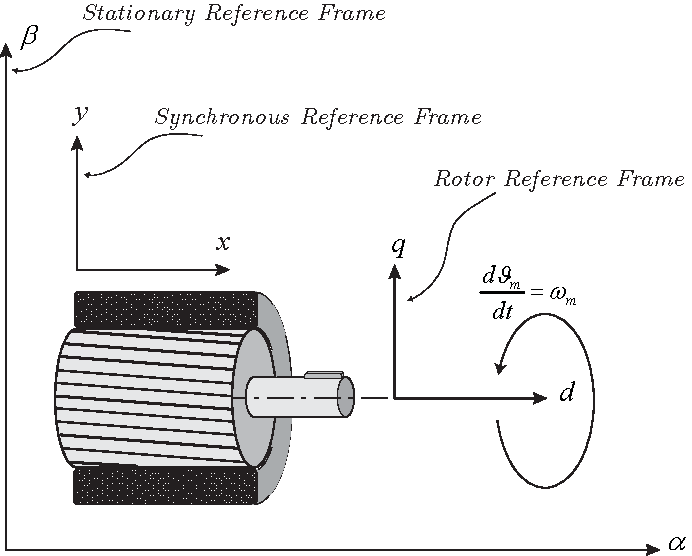
\includegraphics[width = 275pt, 
	keepaspectratio]{figures/kalman/im_reference_frames_3.pdf}
	\captionsetup{width=.5\textwidth}
	\caption{Different point of views regarding different reference frames: 
		stationary $(\alpha,\beta)$ can be considered in still condition; rotor 
		$(d,q)$ can be thought rotating at the rotor speed; synchronous 
		reference 
		frame $(x,y)$ can be thought rotating at electrical stator pulsation.}
	\label{figure_im_ref_frame2} 
\end{figure}
%\begin{figure}[H]
%	\centering
%	\includegraphics[width = 200pt, 
%	keepaspectratio]{figures/kalman/im_pic.jpg}
%	\captionsetup{width=.5\textwidth}
%	\caption{Internal view of a typical induction motor with squirrel cage 
%		rotor.}
%	\label{figure_im_machine_view} 
%\end{figure}

As we have seen, stator flux equations are represented respect the stationary 
reference frame while the rotor flux equations are represented respect to the 
rotor reference frame. Now we want to transform the rotor flux equations from 
the rotor to the stationary reference frame. 

Considering that
\begin{equation}\label{im_eq_15}
	\frac{d\mathbf{T}_2(\vartheta_m)}{dt}= 
	-\omega_m\mathbf{T}_2(\vartheta_m)\begin{pmatrix} 0 & -1\\ 1 & 0 
	\end{pmatrix} = -\omega_m\begin{pmatrix} 0 & -1\\ 1 & 0 \end{pmatrix} 
	\mathbf{T}_2(\vartheta_m)
\end{equation}
\begin{equation}\label{im_eq_16}
	\frac{d\mathbf{T}_2^{-1}(\vartheta_m)}{dt}= 
	-\omega_m\mathbf{T}_2^{-1}(\vartheta_m)\begin{pmatrix} 0 & 1\\ -1 & 0 
	\end{pmatrix} = -\omega_m\begin{pmatrix} 0 & 1\\ -1 & 0 \end{pmatrix} 
	\mathbf{T}_2^{-1}(\vartheta_m)
\end{equation}

The rotor flux equations respect to the stationary reference frame become as 
follows
\begin{equation}\label{im_eq_17}
	\begin{aligned}
		\dot{\vec{\psi}}_{dq}^{\,r}=\frac{d}{dt}\Bigg(\mathbf{T}_2(\vartheta_m) 
		{\vec{\psi}}_{\alpha\beta}^{\,r}\Bigg)&=-\omega_m\begin{pmatrix}
			0&-1\\1&0\end{pmatrix}\mathbf{T}_2(\vartheta_m){\vec{\psi}}_{\alpha\beta}^{\,r}
		+\mathbf{T}_2(\vartheta_m)\dot{\vec{\psi}}_{\alpha\beta}^{\,r}\\[8pt]
		&=-\mathbf{R}_r\mathbf{T}_2(\vartheta_m){\vec{i}}_{\alpha\beta}^{\,r}
	\end{aligned}
\end{equation}
multiplying left side by $\mathbf{T}_2^{-1}(\vartheta_m)$ we obtain
\begin{equation}\label{im_eq_18}
	\begin{aligned}
		\dot{\vec{\psi}}_{\alpha\beta}^{\,r}=\omega_m\begin{pmatrix} 
			0&-1\\1&0\end{pmatrix} 
		{\vec{\psi}}_{\alpha\beta}^{\,r}-\mathbf{R}_r{\vec{i}}_{\alpha\beta}^{\,r}
	\end{aligned}
\end{equation}
or
\begin{equation}\label{im_eq_19}
	\begin{aligned}
		\left[
		\begin{matrix}
			\dot{\psi}_{r\alpha} \\[6pt]
			\dot{\psi}_{r\beta}
		\end{matrix} \right] = -
		\left[
		\begin{matrix}
			R_r & 0 \\[6pt]
			0 & R_r 
		\end{matrix} \right]
		\left[
		\begin{matrix}
			i_{r\alpha} \\[6pt]
			i_{r\beta}
		\end{matrix} \right] - 
		\left[
		\begin{matrix}
			0 & \omega_m \\[6pt]
			- \omega_m & 0
		\end{matrix} \right]
		\left[
		\begin{matrix}
			{\psi}_{r\alpha} \\[6pt]
			{\psi}_{r\beta}
		\end{matrix} \right]
	\end{aligned}
\end{equation}


%\begin{equation} \label{eq36}
%\begin{aligned}
%\left[
%\begin{matrix}
%\dot{\psi}_{r\alpha} \\
%\dot{\psi}_{r\beta}
%\end{matrix} \right] = &
%\left[
%\begin{matrix}
%\cos\vartheta_m & \sin\vartheta_m \\
%-\sin\vartheta_m & \cos\vartheta_m \\
%\end{matrix} \right]
%\left[
%\begin{matrix}
%\dot{\psi}_{rd} \\
%\dot{\psi}_{rq}
%\end{matrix} \right] - \omega_m
%\left[
%\begin{matrix}
%\sin\vartheta_m & \cos\vartheta_m \\
%-\cos\vartheta_m & \sin\vartheta_m \\
%\end{matrix} \right]
%\left[
%\begin{matrix}
%\psi_{rd} \\
%\psi_{rq}
%\end{matrix} \right] \\[6pt]
%= & -
%\left[
%\begin{matrix}
%R_r & 0 \\
%0 & R_r \\
%\end{matrix} \right]
%\left[
%\begin{matrix}
%i_{r\alpha} \\
%i_{r\beta}
%\end{matrix} \right] + 
%\left[
%\begin{matrix}
%-\omega_m{\psi}_{r\beta} \\
%\omega_m{\psi}_{r\alpha}
%\end{matrix} \right]
%\end{aligned}
%\end{equation}
Now we can write all terms of the Eq.~\eqref{im_eq_11} in $(\alpha,\,\beta)$ 
coordinates as follows
\begin{equation} \label{im_eq_20}
	\begin{aligned}
		&\left[
		\begin{matrix}
			\dot{\psi}_{s\alpha} \\[6pt]
			\dot{\psi}_{s\beta}
		\end{matrix} \right] = -
		\left[
		\begin{matrix}
			R_s & 0 \\[6pt]
			0 & R_s 
		\end{matrix} \right]
		\left[
		\begin{matrix}
			i_{s\alpha} \\[6pt]
			i_{s\beta}
		\end{matrix} \right] +
		\left[
		\begin{matrix}
			u_{s\alpha} \\[6pt]
			u_{s\beta}
		\end{matrix}
		\right] \\[6pt]
		&\left[
		\begin{matrix}
			\dot{\psi}_{r\alpha} \\[6pt]
			\dot{\psi}_{r\beta}
		\end{matrix} \right] = -
		\left[
		\begin{matrix}
			R_r & 0 \\[6pt]
			0 & R_r
		\end{matrix} \right]
		\left[
		\begin{matrix}
			i_{r\alpha} \\[6pt]
			i_{r\beta}
		\end{matrix} \right] - 
		\left[
		\begin{matrix}
			0 & \omega_m \\[6pt]
			- \omega_m & 0
		\end{matrix} \right]
		\left[
		\begin{matrix}
			{\psi}_{r\alpha} \\[6pt]
			{\psi}_{r\beta}
		\end{matrix} \right]
	\end{aligned}
\end{equation}

The electromagnetic equations are
\begin{equation}\label{im_eq_21}
	\left[\begin{matrix}
		\psi_{s\alpha} \\[6pt]
		\psi_{s\beta} \\[6pt]
		\psi_{r\alpha} \\[6pt]
		\psi_{r\beta}
	\end{matrix}\right] = 
	\left[\begin{matrix}
		L_s & 0 & L_m & 0 \\[6pt]
		0 & L_s & 0 & L_m \\[6pt]
		L_m & 0 & L_r & 0 \\[6pt]
		0 & L_m & 0 & L_r 
	\end{matrix}\right]
	\left[\begin{matrix}
		i_{s\alpha} \\[6pt]
		i_{s\beta} \\[6pt]
		i_{r\alpha} \\[6pt]
		i_{r\beta} 
	\end{matrix}\right] = \mathbf{L}
	\left[\begin{matrix}
		i_{s\alpha} \\[6pt]
		i_{s\beta} \\[6pt]
		i_{r\alpha} \\[6pt]
		i_{r\beta} 
	\end{matrix}\right]
\end{equation}
i.e. the quadratic form associated to $\mathbf{L}$
\begin{equation}\label{im_eq_22}
	\frac{3}{2}\Bigg(\frac{1}{2}\vec{i}_{\alpha\beta}^{\,\,T} 
	\,\mathbf{L}\vec{i}_{\alpha\beta}\Bigg)
\end{equation}
is positive for any non-zero value of the current vector 
$\vec{i}_{\alpha\beta}=[i_{s\alpha},\,i_{s\beta},\,i_{r\alpha},\,i_{r\beta}]$ 
and represent the magnetic energy.

Define 
\begin{equation}\label{im_eq_23}
	\mathbf{R}=
	\left[\begin{matrix}
		R_s & 0 & 0 & 0 \\[6pt]
		0 & R_s & 0 & 0 \\[6pt]
		0 & 0 & R_r & 0 \\[6pt]
		0 & 0 & 0 & R_r 
	\end{matrix}\right]
\end{equation}
the state space model representation of the system Eq.~\eqref{im_eq_20} is
\begin{equation}\label{im_eq_24}
	\begin{aligned}
		\mathbf{L} &
		\begin{bmatrix}
			\frac{d}{dt} i_{s\alpha} \\[6pt]
			\frac{d}{dt} i_{s\beta} \\[6pt]
			\frac{d}{dt} i_{r\alpha} \\[6pt]
			\frac{d}{dt} i_{r\beta}
		\end{bmatrix} = -\mathbf{R}
		\begin{bmatrix}
			i_{s\alpha} \\[6pt]
			i_{s\beta} \\[6pt]
			i_{r\alpha} \\[6pt]
			i_{r\beta} 
		\end{bmatrix} + \\[6pt]
		+ &
		\begin{bmatrix}
			0 & 0 & 0 & 0 \\[6pt]
			0 & 0 & 0 & 0 \\[6pt]
			0 & \omega_mL_m & 0 & \omega_mL_r \\[8pt]
			-\omega_mL_m & 0 & -\omega_mL_r & 0
		\end{bmatrix}
		\begin{bmatrix}
			i_{s\alpha} \\[6pt]
			i_{s\beta} \\[6pt]
			i_{r\alpha} \\[6pt]
			i_{r\beta} 
		\end{bmatrix} + 
		\begin{bmatrix}
			u_{s\alpha} \\[6pt]
			u_{s\beta} \\[6pt]
			0 \\[6pt]
			0
		\end{bmatrix} \\[8pt]
		&
		J\frac{d}{dt}{\omega}_m = \tau_e-\tau_l
	\end{aligned}
\end{equation}
in which the state variables are $(i_{s\alpha},\,i_{s\beta}, 
i_{r\alpha},\,i_{r\beta},\,\omega_m)$ and the electromagnetic torque $\tau_e$ 
is still to be determined as a function of the state variables. This choice of 
state variables is naturally linked to the energy stored in the energy stored 
in the motor given by
\begin{equation}\label{im_eq_25}
	E = \frac{3}{2}\Bigg(\frac{1}{2} \vec{i}_{\alpha\beta}^{\,\,T} 
	\,\mathbf{L}\, \vec{i}_{\alpha\beta} \Bigg)+\frac{1}{2}J\omega_m^2
\end{equation}
which is the sum of the magnetic energy and of the kinetic energy
\begin{equation}\label{im_eq_26}
	\frac{1}{2}J\omega_m^2
\end{equation}
The expression of $\tau_e$ can be obtained from the energy balance
\begin{equation}\label{im_eq_27}
	\begin{aligned}
		\frac{dE}{dt} = &
		\frac{3}{2}\left[\begin{matrix}
			i_{s\alpha} & i_{s\beta}
		\end{matrix}\right]
		\left[\begin{matrix}
			u_{s\alpha} & u_{s\beta}
		\end{matrix}\right]^T 
		-\tau_l\,\omega_m-\frac{3}{2}\vec{i}_{\alpha\beta}^{\,\,T}\mathbf{R}\vec{i}_{\alpha\beta}
		+ \\[6pt]
		& + \frac{3}{2}\omega_m
		\left[\begin{matrix}
			i_{r\alpha} & i_{r\beta}
		\end{matrix}\right]
		\left[\begin{matrix}
			0 & -L_m \\
			L_m & 0
		\end{matrix}\right]
		\left[\begin{matrix}
			i_{s\alpha} & i_{s\beta}
		\end{matrix}\right]^T
		+\tau_e\omega_m
	\end{aligned}
\end{equation}
Let $P_{in}$, $P_{out}$ and $P_{loss}$ denote the input power, the output 
power, and the power losses, respectively; since
\begin{equation}\label{im_eq_28}
	\begin{aligned}
		\frac{dE}{dt} = & P_{in} - P_{out} -P_{loss} \\[6pt]
		= &
		\frac{3}{2}\left[\begin{matrix}
			i_{s\alpha} & i_{s\beta}
		\end{matrix}\right]
		\left[\begin{matrix}
			u_{s\alpha} & u_{s\beta}
		\end{matrix}\right]^T 
		-\tau_l\,\omega_m-\frac{3}{2}\vec{i}_{\alpha\beta}^{\,\,T}\mathbf{R}\vec{i}_{\alpha\beta}
	\end{aligned}
\end{equation}
which means 
\begin{equation}\label{im_eq_29}
	\tau_e = 
	\frac{3}{2}\left[\begin{matrix}
		i_{r\alpha} & i_{r\beta}
	\end{matrix}\right]
	\left[\begin{matrix}
		0 & -L_m \\
		L_m & 0
	\end{matrix}\right]
	\left[\begin{matrix}
		i_{s\alpha} & i_{s\beta}
	\end{matrix}\right]^T = 
	\frac{3}{2}L_m\left(i_{r\alpha} i_{s\beta} - i_{r\beta} i_{s\alpha}\right)
\end{equation}
Note that the electromagnetic torque $\tau_e$ produced by the motor is a 
non-linear function of the state variables and constitutes the main non-linear 
term in the induction motor model. Since
\begin{equation}\label{im_eq_30}
	\begin{aligned}
		i_{r\alpha} &= -\frac{L_m}{L_r}i_{s\alpha}+\frac{1}{Lr}\psi_{r\alpha} 
		\\[8pt]
		i_{r\beta} &= -\frac{L_m}{L_r}i_{s\beta}+\frac{1}{Lr}\psi_{r\beta}
	\end{aligned}
\end{equation}
the electromagnetic torque can be expressed as
\begin{equation}\label{im_eq_31}
	\tau_{e} = 
	\frac{3}{2}\frac{L_m}{L_r}\left(\psi_{r\alpha}i_{s\beta}-\psi_{r\beta}i_{s\alpha}\right).
\end{equation}
Eliminating $\left(\psi_{s\alpha}, \psi_{s\beta}, i_{r\alpha}, 
i_{r\beta}\right)$ from equation  \ref{im_eq_20} using equations \ref{im_eq_20} 
and \ref{im_eq_30}, namely
\begin{equation}\label{im_eq_32}
	\left[\begin{matrix}
		i_{r\alpha} \\[6pt]
		i_{r\beta}
	\end{matrix}\right] = 
	\left[\begin{matrix}
		-\frac{L_m}{L_r} & 0 \\[6pt]
		0 & -\frac{L_m}{L_r}
	\end{matrix}\right]
	\left[\begin{matrix}
		i_{s\alpha} \\[6pt]
		i_{s\beta}
	\end{matrix}\right]+
	\left[\begin{matrix}
		\frac{1}{L_r} & 0 \\[6pt]
		0 & \frac{1}{L_r}
	\end{matrix}\right]
	\left[\begin{matrix}
		\psi_{r\alpha} \\[6pt]
		\psi_{r\beta}
	\end{matrix}\right]\\[6pt]
\end{equation}
\begin{equation}\label{eq51}
	\left[\begin{matrix}
		\psi_{s\alpha} \\[6pt]
		\psi_{s\beta}
	\end{matrix}\right] = 
	\left[\begin{matrix}
		L_s-\frac{L_m^2}{L_r} & 0 \\[6pt]
		0 & L_s-\frac{L_m^2}{L_r}
	\end{matrix}\right]
	\left[\begin{matrix}
		i_{s\alpha} \\[6pt]
		i_{s\beta}
	\end{matrix}\right]+
	\left[\begin{matrix}
		\frac{L_m}{L_r} & 0 \\[6pt]
		0 & \frac{L_m}{L_r}
	\end{matrix}\right]
	\left[\begin{matrix}
		\psi_{r\alpha} \\[6pt]
		\psi_{r\beta}
	\end{matrix}\right]
\end{equation}
we obtain a state model in terms of the state variables 
$\left(\omega_m,\,\psi_{r\alpha},\, 
\psi_{r\beta},\,i_{s\alpha},\,i_{s\beta}\right)^T$, the input variables 
$\left(u_{s\alpha},\, u_{s\beta}\right)^T$ and the disturbance $\tau_l$

\begin{mybox}
	\textbf{IM Dynamical Model Respect to a Stationary Reference Frame}
	\begin{equation}\label{im_eq_33}
		\begin{aligned}
			\frac{di_{s\alpha}}{dt} &= -\gamma i_{s\alpha}  + 
			\beta\alpha\psi_{r\alpha}+\beta\omega_m\psi_{r\beta} + 
			\frac{u_{s\alpha}}{\sigma}\\[6pt]
			\frac{di_{s\beta}}{dt} &= -\gamma i_{s\beta}  + 
			\beta\alpha\psi_{r\beta}-\beta\omega_m\psi_{r\alpha} + 
			\frac{u_{s\beta}}{\sigma} \\[6pt]
			\frac{d\psi_{r\alpha}}{dt} &= -\alpha \psi_{r\alpha} 
			-\omega_m\psi_{r\beta}+\alpha L_m i_{s\alpha} \\[6pt]
			\frac{d\psi_{r\beta}}{dt} &= -\alpha \psi_{r\beta} 
			+\omega_m\psi_{r\alpha}+\alpha L_m i_{s\beta} \\[6pt]
			\frac{d\omega_m}{dt} &= \mu \left(\psi_{r\alpha}i_{s\beta} - 
			\psi_{r\beta}i_{s\alpha}\right)-\frac{\tau_l}{J}
		\end{aligned}
	\end{equation}
	\textbf{where}
	\begin{equation}\label{im_eq_34}
		\begin{aligned}
			\mu & = \frac{3}{2}\frac{L_m}{JL_r}, \quad
			\alpha = \frac{R_r}{L_r},  \quad
			\sigma = L_s \left(1-\frac{L_m^2}{L_sL_r}\right) \\[6pt]
			\beta & = \frac{L_m}{\sigma L_r},  \quad
			\gamma = \frac{R_s}{\sigma} + \beta \alpha L_m
		\end{aligned}
	\end{equation}
\end{mybox}
Consider now the condition of constant speed
\begin{equation}\label{im_eq_35}
	\frac{d\omega_m}{dt}=0 \quad\Rightarrow\quad\omega_m=\omega_m^0
\end{equation}
which brings the above system from a nonlinear time-variant into a linear 
time-invariant as shown in the following
\begin{mybox}
	\textbf{IM Dynamical Model Respect to a Stationary Reference Frame and 
		Constant Rotor Speed}
	\begin{equation}\label{im_eq_36}
		\begin{aligned}
			\dot{\vec{x}} &=\tilde{\mathbf{A}}\vec{x}+\tilde{\mathbf{B}}\vec{u} 
			\\[6pt]
			{\vec{y}} &={\mathbf{C}}\vec{x}
		\end{aligned}
	\end{equation}
	where
	\begin{equation}\label{im_eq_37}
		\begin{aligned}
			&\vec{x} = \begin{bmatrix} 
				i_{s\alpha}&i_{s\beta}&\psi_{r\alpha}&\psi_{r\beta} 
			\end{bmatrix}^T\\[6pt]
			&\vec{u} = \begin{bmatrix} u_{s\alpha}&u_{s\beta} 
			\end{bmatrix}^T\\[6pt]
			&\vec{y} = \begin{bmatrix} i_{s\alpha}&i_{s\beta} 
			\end{bmatrix}^T\\[6pt]
			&\tilde{\mathbf{A}} = \begin{bmatrix}
				-\gamma&0&\beta\alpha&\beta\omega_m^0 \\[6pt]			
				0&-\gamma&-\beta\omega_m^0&\beta\alpha \\[6pt]
				\alpha L_m&0&-\alpha&-\omega_m^0 \\[6pt]
				0&\alpha L_m&\omega_m^0&-\alpha \\[6pt]
			\end{bmatrix},\qquad
			\tilde{\mathbf{B}} = \begin{bmatrix}
				\frac{1}{\sigma}&0 \\[6pt]			
				0&\frac{1}{\sigma} \\[6pt]
				0&0 \\[6pt]
				0&0 \\[6pt]
			\end{bmatrix} \\[6pt]
			&\mathbf{C} = \begin{bmatrix}
				1&0&0&0 \\[6pt]			
				0&1&0&0	
			\end{bmatrix}
		\end{aligned}
	\end{equation}
	\textbf{The expression of the electromagnetic torque is as follows}
	\begin{equation}\label{im_eq_38}
		\tau_e = \frac{3}{2}\frac{L_m}{L_r}\Big(\psi_{r\alpha}i_{s\beta} - 
		\psi_{r\beta}i_{s\alpha}\Big)
	\end{equation}
\end{mybox}

The state space model \ref{im_eq_33}, which will be referred to as fixed frame 
model, has some advantages from the control view point since it clarifies that 
the control inputs $\left(u_{s\alpha},\, u_{s\beta}\right)$ directly affect the 
dynamics of the stator currents $\left(i_{s\alpha},\, i_{s\beta}\right)$ which 
can be viewed as immediate control variables since they control the rotor speed 
$\omega_m$ and the rotor flux modulus $\sqrt{\psi_{r\alpha}^2 + 
	\psi_{r\beta}^2}$ in the first three equations.

Let us now introduce a time-varing $\left(d,\,q\right)$ frame which rotates at 
an arbitrary speed $\omega_0(t)$ and is identified at each time $t$ by the 
angle $\vartheta_0(t)$ so that
\begin{equation}\label{im_eq_39}
	\frac{d\vartheta_0}{dt} = \omega_0
\end{equation}
Rotor fluxes $(\psi_{r\alpha},\,\psi_{r\beta})$, stator currents 
$(i_{s\alpha},\,i_{s\beta})$, and stator voltages $(u_{s\alpha},\,u_{s\beta})$ 
are expressed with respect to the time-varying rotating $(d,\,q)$ frame as 
\begin{equation}\label{im_eq_40}
	\begin{aligned}
		\left[
		\begin{matrix}
			\psi_{rd} \\[6pt]
			\psi_{rq}
		\end{matrix}
		\right] & =
		\left[
		\begin{matrix}
			\cos\vartheta_0 & \sin\vartheta_0 \\[6pt]
			-\sin\vartheta_0 & \cos\vartheta_0 
		\end{matrix}
		\right]
		\left[
		\begin{matrix}
			\psi_{r\alpha} \\[6pt]
			\psi_{r\beta}
		\end{matrix}
		\right] \\[6pt]
		\left[
		\begin{matrix}
			i_{sd} \\[6pt]
			i_{sq}
		\end{matrix}
		\right] & =
		\left[
		\begin{matrix}
			\cos\vartheta_0 & \sin\vartheta_0 \\[6pt]
			-\sin\vartheta_0 & \cos\vartheta_0 
		\end{matrix}
		\right]
		\left[
		\begin{matrix}
			i_{s\alpha} \\[6pt]
			i_{s\beta}
		\end{matrix}
		\right] \\[6pt]
		\left[
		\begin{matrix}
			u_{sd} \\[6pt]
			u_{sq}
		\end{matrix} 
		\right] & = 
		\left[
		\begin{matrix}
			\cos\vartheta_0 & \sin\vartheta_0 \\[6pt]
			-\sin\vartheta_0 & \cos\vartheta_0
		\end{matrix}
		\right]
		\left[
		\begin{matrix}
			u_{s\alpha} \\[6pt]
			u_{s\beta}
		\end{matrix}
		\right]
	\end{aligned}
\end{equation}
If the new \textbf{state variables} 
$(\omega_m,\,\psi_{rd},\,\psi_{rq},\,i_{sd},\,i_{sq})^T$ and input variables 
$(u_{sd},\,u_{sq})$ are used, in the new $(d,\,q)$ rotating coordinates the 
induction motor model becomes; consider the quantity $\tau_l$ as disturbance.
\begin{mybox}
	\textbf{IM Dynamical Model Respect to a Rotating Reference Frame}
	\begin{equation}\label{im_eq_41}
		\begin{aligned}
			\frac{d\omega_m}{dt} &= \mu \left(\psi_{rd}i_{sq} - 
			\psi_{rq}i_{sd}\right)-\frac{\tau_l}{J} \\[6pt]
			\frac{d\psi_{rd}}{dt} &= -\alpha \psi_{rd} 
			+\left(\omega_0-\omega_m\right) \psi_{rq}+ \alpha L_m i_{sd} \\[6pt]
			\frac{d\psi_{rq}}{dt} &= -\alpha 
			\psi_{rq}-\left(\omega_0-\omega_m\right) \psi_{rd}+\alpha L_m 
			i_{sq} \\[6pt]
			\frac{di_{sd}}{dt} &= -\gamma i_{sd}  + \omega_0 i_{sq} + 
			\beta\alpha\psi_{rd}+\beta\omega_m\psi_{rq} + \frac{u_{sd}}{\sigma} 
			\\[6pt]
			\frac{di_{sq}}{dt} &= -\gamma i_{sq}  - \omega_0 i_{sd} + 
			\beta\alpha\psi_{rq}-\beta\omega_m\psi_{rd} + \frac{u_{sq}}{\sigma}
		\end{aligned}
	\end{equation}
	where $\omega_0$ is the speed of the rotating reference frame
	\textbf{where}
	\begin{equation}\label{im_eq_42}
		\begin{aligned}
			\mu & = \frac{3}{2}\frac{L_m}{JL_r}, \quad
			\alpha = \frac{R_r}{L_r},  \quad
			\sigma = L_s \left(1-\frac{L_m^2}{L_sL_r}\right) \\[6pt]
			\beta & = \frac{L_m}{\sigma L_r},  \quad
			\gamma = \frac{R_s}{\sigma} + \beta \alpha L_m
		\end{aligned}
	\end{equation}
\end{mybox}

In the case the rotating reference is attached to the rotor the induction motor 
model becomes
\begin{mybox}
	\textbf{IM Dynamical Model Respect to the Rotor Reference Frame}
	\begin{equation}\label{im_eq_43}
		\begin{aligned}
			\frac{d\omega_m}{dt} &= \mu \left(\psi_{rd}i_{sq} - 
			\psi_{rq}i_{sd}\right)-\frac{\tau_l}{J} \\[6pt]
			\frac{d\psi_{rd}}{dt} &= -\alpha \psi_{rd} + \alpha L_m i_{sd} 
			\\[6pt]
			\frac{d\psi_{rq}}{dt} &= -\alpha \psi_{rq} + \alpha L_m i_{sq} 
			\\[6pt]
			\frac{di_{sd}}{dt} &= -\gamma i_{sd}  + \omega_m i_{sq} + 
			\beta\alpha\psi_{rd}+\beta\omega_m\psi_{rq} + \frac{u_{sd}}{\sigma} 
			\\[6pt]
			\frac{di_{sq}}{dt} &= -\gamma i_{sq}  - \omega_m i_{sd} + 
			\beta\alpha\psi_{rq}-\beta\omega_m\psi_{rd} + \frac{u_{sq}}{\sigma} 
			\\[6pt]
		\end{aligned}
	\end{equation}
	\textbf{The rotor frame state space model has some advantages from 
		observability view point given by the linearity of the rotor flux 
		equation 
		where the cross terms are deleted from the selected rotating reference 
		frame.}
\end{mybox}

\subsubsection{Model discretization}
As already mentioned, in order to implement our control structure a discrete-time representation 
of the system of Eq.~\eqref{pmsm_problem_1_eq_2} shall be derived. By the use of 
the Euler approximation for the derivatives using the sampling time $t_s$, that is 
\begin{equation}\label{pmsm_problem_1_eq_3}
	\frac{d}{dt}x(t)\approx\frac{x[(k+1)t_s]-x(kt_s)}{t_s}=\frac{x(k+1)-x(k)}{t_s}
\end{equation}
we obtain the following discrete time representation of the PMSM model
\begin{mybox}
	\textbf{Discrete-time representation of the PMSM}
	\begin{equation}\label{pmsm_problem_1_eq_4}
		\left\lbrace \begin{aligned}
			& i_\alpha(k+1)=\Big(1-t_s\frac{R_s}{L_\alpha}\Big) i_\alpha(k) 
			+t_s\frac{\omega(k)}{L_\alpha}\psi_\beta(k)+\frac{t_s}{L_\alpha}u_\alpha(k)
			\\[6pt]
			& i_\beta(k+1) = \Big(1-t_s\frac{R_s}{L_\beta}\Big)i_\beta(k) 
			-t_s\frac{\omega(k)}{L_\beta}\psi_\alpha(k)+\frac{t_s}{L_\beta}u_\beta(k)
			\\[6pt]
			&\psi_\alpha^r(k+1) = \psi_\alpha^r(k) -t_s\omega(k)\psi_\beta^r(k) 
			\\[6pt]
			&\psi_\beta^r(k+1) = \psi_\beta^r(k) + t_s\omega(k)\psi_\alpha^r(k) 
			\\[6pt]
			&\omega_m(k+1) = \omega_m(k) + \frac{t_s}{J}\Bigg[\frac{3}{2}p 
			\Big[\psi^r_{\alpha}(k)i_{\beta}(k)-\psi^r_{\beta}(k)i_{\alpha}(k)\Big] 
			-\tau_l(k) -b{\omega}_m(k) \Bigg]\\[6pt]
			& {\theta}(k+1) = {\theta}(k) + t_s\omega(k) ={\theta}(k) + t_s 
			p\omega_m(k)
		\end{aligned} \right. 
	\end{equation}
	where $p$ is the number of poles pairs, $b$ the bearing viscosity and 
	$\tau_l(t)$ the external and unknown load (disturbance).
\end{mybox}
The model of Eq.~\eqref{pmsm_problem_1_eq_4} can be used to implement the MPC as well as the EKF, anyway to implement the EKF we proceed in a little bit different way: we first propose a linearization of Eq.~\eqref{pmsm_problem_1_eq_2} along the estimated state vector $\hat{\vec{x}}$ (where we obtain a linear model) and after that we discretize by Taylor as already seen. This procedure will be described in section~\ref{PMSM_EKF}



\subsection{Extended Kalman Filter (EKF) Observer}\label{PMSM_EKF}
In this section an application of the Extended Kalman filter is presented, where a PMSM rotor fluxes estimator is proposed and implemented. We will proceed using the  $\alpha\beta$ model representation reported in Eq.~\eqref{pmsm_problem_1_eq_2}. 

A different, but equivalent, representation of the PMSM can be re-written as follows
\begin{equation}\label{pmsm_problem_1_eq_5}
	\left\lbrace \begin{aligned}
		&\frac{d}{dt}\vec{x}(t)=\vec{g}(\vec{x})+\mathbf{B}\vec{u}(t)
		\\[6pt]
		&\vec{y}(t) = \mathbf{C}\vec{x}(t)
	\end{aligned}\right. 
\end{equation} 
where 
\begin{equation}\label{pmsm_problem_1_eq_6}
	\begin{aligned}
		\vec{x}=\begin{bmatrix} i_\alpha \\[6pt] i_\beta \\[6pt] \psi_\alpha^r 
			\\[6pt] \psi_\beta^r \\[6pt] \vartheta \\[6pt] \omega \end{bmatrix},\quad
		\vec{u}=\begin{bmatrix} u_\alpha \\[6pt] u_\beta \end{bmatrix}
	\end{aligned}
\end{equation}
and where
\begin{equation}\label{pmsm_problem_1_eq_7}
	\begin{aligned}
		\mathbf{B} = \frac{1}{L_s}\begin{bmatrix} 1&0 \\[6pt] 
			0&1\\[6pt] 0&0 \\[6pt] 0&0  \end{bmatrix},\quad
		\mathbf{C} = \begin{bmatrix} 1&0&0&0&0&0 \\[6pt] 0&1&0&0&0&0 
		\end{bmatrix}
	\end{aligned}
\end{equation} 
and where
\begin{align}\label{pmsm_problem_1_eq_8}
	\frac{d}{dt}\vec{x}(t)=\vec{g}(\vec{x})\Rightarrow\left\lbrace 
	\begin{aligned}
		\begin{split}
			&\frac{d}{dt}i_\alpha(t) = -\frac{R_s}{L_s}i_\alpha(t) + 	
			\frac{1}{L_s}\omega(t)\psi_\beta^r(t) + \frac{1}{L_s} u_\alpha(t) 
		\end{split}	\\[6pt]
		\begin{split}
			&\frac{d}{dt}i_\beta(t) = -\frac{R_s}{L_s}i_\beta(t) - 	
			\frac{1}{L_s}\omega(t)\psi_\alpha^r(t) + \frac{1}{L_s} u_\beta(t)	
		\end{split}	\\[6pt]
		\begin{split}
			&\frac{d}{dt}\psi_\alpha^r(t) = -\omega(t)\psi_\beta^r(t)
		\end{split}	\\[6pt]
		\begin{split}	
			&\frac{d}{dt}\psi_\beta^r(t) = \omega(t)\psi_\alpha^r(t)	
		\end{split}	\\[6pt]
		\begin{split}
			&\frac{d}{dt}\vartheta(t) = \omega(t)
		\end{split}	\\[6pt]
		\begin{split}
			&\frac{d}{dt}\omega(t) = 
			\frac{1}{J}\Bigg[\frac{3}{2}\Big(\psi^r_{\alpha}(t)i_{\beta}(t) - 
			\psi^r_{\beta}(t)i_{\alpha}(t)\Big)  -\frac{1}{p}\tau_l(t) 
			-\frac{1}{p}b\omega_m(t)\Bigg]
		\end{split}
	\end{aligned}\right. 
\end{align}
we are considering $L_\alpha = \L_\beta = L_s$.

\vspace{5mm}
\textbf{For the purpose of the EKF implementation a reduced dynamic description is 
	taken into account}, in particular it is assumed the dynamic of the mechanical 
system is more then one order slower than the electrical system and for this 
assumption we decide to represent the system of Eq.~\eqref{pmsm_problem_1_eq_8} as follows
\begin{align}\label{pmsm_problem_1_eq_9}
	\frac{d}{dt}\vec{x}(t)=\vec{f}(\vec{x})\Rightarrow\left\lbrace 
	\begin{aligned}
		\begin{split}
			&\frac{d}{dt}i_\alpha(t) = -\frac{R_s}{L_s}i_\alpha(t) + 	
			\frac{1}{L_s}\omega(t)\psi_\beta^r(t) + \frac{1}{L_s} u_\alpha(t) 
		\end{split}	\\[6pt]
		\begin{split}
			&\frac{d}{dt}i_\beta(t) = -\frac{R_s}{L_s}i_\beta(t) - 	
			\frac{1}{L_s}\omega(t)\psi_\alpha^r(t) + \frac{1}{L_s} u_\beta(t)	
		\end{split}	\\[6pt]
		\begin{split}
			&\frac{d}{dt}\psi_\alpha^r(t) = -\omega(t)\psi_\beta^r(t)
		\end{split}	\\[6pt]
		\begin{split}	
			&\frac{d}{dt}\psi_\beta^r(t) = \omega(t)\psi_\alpha^r(t)	
		\end{split}	\\[6pt]
		\begin{split}
			&\frac{d}{dt}\vartheta(t) = \omega(t)
		\end{split}	\\[6pt]
		\begin{split}
			&\frac{d}{dt}\omega(t) = 0
		\end{split}
	\end{aligned}\right. 
\end{align}
where the mechanical dynamic has been \textbf{intentionally} approximated to a 
stationary motion.
\begin{mybox}
	In order to implement the EKF we now linearize the system of Eq.~\eqref{pmsm_problem_1_eq_9} along the estimated state space trajectory $\hat{\vec{x}}$, as follows
	\begin{equation}\label{pmsm_problem_1_eq_10}
		\begin{aligned}
			\left.\frac{\partial}{\partial 
				\vec{x}}\vec{f}(\vec{x})\right|_{\vec{x}=\hat{\vec{x}}} &= 
			\begin{bmatrix} \frac{\partial f_1}{\partial x_1} & \cdots & 
				\frac{\partial f_1}{\partial x_n} \\[6pt]
				\vdots & \ddots & \vdots \\[6pt]
				\frac{\partial f_n}{\partial x_1} & \cdots & \frac{\partial 
					f_n}{\partial x_n}
			\end{bmatrix}_{\hat{\vec{x}}(t)} = \tilde{\mathbf{A}}_1 + 
			\hat{\omega}(t) \tilde{\mathbf{A}}_2 + \hat{\psi}_\alpha^r(t) 
			\tilde{\mathbf{A}}_3 + \hat{\psi}_\beta^r(t) \tilde{\mathbf{A}}_4 = 
			\tilde{\mathbf{A}}(t)
		\end{aligned}
	\end{equation} 
	where $\hat{\vec{x}}$ is the estimated state vector from the EKF.
\end{mybox}

The matrices $\tilde{\mathbf{A}}_1$, $\tilde{\mathbf{A}}_2$, 
$\tilde{\mathbf{A}}_3$ and $\tilde{\mathbf{A}}_4$ are as follows
\begin{equation}\label{pmsm_problem_1_eq_11}
	\begin{aligned}
		&\tilde{\mathbf{A}}_1 = 
		\begin{bmatrix} 
			-\frac{R_s}{L_s} & 0 & 0 & 0 & 0 & 0 \\[6pt]			
			0 & -\frac{R_s}{L_s} & 0 & 0 & 0 & 0 \\[6pt]
			0 & 0 & 0 & 0 & 0 & 0 \\[6pt]
			0 & 0 & 0 & 0 & 0 & 0 \\[6pt]
			0 & 0 & 0 & 0 & 0 & 1 \\[6pt]
			0 & 0 & 0 & 0 & 0 & 0
		\end{bmatrix},\quad
		\tilde{\mathbf{A}}_2 = 
		\begin{bmatrix} 
			0 & 0 & 0 & \frac{1}{L_s} & 0 & 0 \\[6pt]			
			0 & 0 & -\frac{1}{L_s} & 0 & 0 & 0 \\[6pt]
			0 & 0 & 0 & -1 & 0 & 0 \\[6pt]
			0 & 0 & 1 & 0 & 0 & 0 \\[6pt]
			0 & 0 & 0 & 0 & 0 & 0 \\[6pt]
			0 & 0 & 0 & 0 & 0 & 0
		\end{bmatrix} \\[8pt]
		&\tilde{\mathbf{A}}_3 = 
		\begin{bmatrix} 
			0 & 0 & 0 & 0 & 0 & 0 \\[6pt]			
			0 & 0 & 0 & 0 & 0 & -\frac{1}{L_s} \\[6pt]
			0 & 0 & 0 & 0 & 0 & 0 \\[6pt]
			0 & 0 & 0 & 0 & 0 & 1 \\[6pt]
			0 & 0 & 0 & 0 & 0 & 0 \\[6pt]
			0 & 0 & 0 & 0 & 0 & 0
		\end{bmatrix},\quad
		\tilde{\mathbf{A}}_4 = 
		\begin{bmatrix} 
			0 & 0 & 0 & 0 & 0 & \frac{1}{L_s} \\[6pt]			
			0 & 0 & 0 & 0 & 0 & 0 \\[6pt]
			0 & 0 & 0 & 0 & 0 & -1 \\[6pt]
			0 & 0 & 0 & 0 & 0 & 0 \\[6pt]
			0 & 0 & 0 & 0 & 0 & 0 \\[6pt]
			0 & 0 & 0 & 0 & 0 & 0
		\end{bmatrix} 
	\end{aligned}
\end{equation} 

The discretization of the transition matrix $\tilde{\mathbf{A}}(t)$ can be 
approximated by Taylor as follows
\begin{equation}\label{pmsm_problem_1_eq_12}
	{\mathbf{A}}(k|k-1) = \mathbf{I} + \tilde{\mathbf{A}}_1t_s + 
	\hat{\omega}(k|k-1) \tilde{\mathbf{A}}_2t_s + \hat{\psi}_\alpha^r(k|k-1) 
	\tilde{\mathbf{A}}_3t_s + \hat{\psi}_\beta^r(k|k-1) \tilde{\mathbf{A}}_4t_s
\end{equation}
The EKF set of equations can be written as follows
\begin{mybox}
	\noindent\textbf{The Extended Kalman Filter Algorithm}
	\begin{align}\label{pmsm_problem_1_eq_13}
		\begin{split}
			&\hat{\vec{x}}\left(k|k\right) = \mathbf{A}(k|k-1) 
			\hat{\vec{x}}\left(k|k-1\right) + \mathbf{B} 
			\vec{u}\left(k|k-1\right)
		\end{split} \\[8pt]
		\begin{split}
			&\mathbf{P}\left(k|k\right) = 
			\mathbf{A}(k|k-1)\mathbf{P}\left(k|k-1\right) \mathbf{A}(k|k-1)^T + 
			\mathbf{Q} 
		\end{split}\\[8pt]
		\begin{split}
			&\mathbf{L}(k) = \mathbf{P}(k|k)\mathbf{C}^{\,T} 
			\Big(\mathbf{C}\,\mathbf{P}(k|k)\,\mathbf{C}^{\,T} 
			+\mathbf{R}\Big)^{-1}
		\end{split}\\[8pt]
		\begin{split}
			&\hat{\vec{x}}\left(k+1|k\right) = \hat{\vec{x}}\left(k|k\right) + 
			\mathbf{L}(k)\, \Big(\vec{y}(k) - 
			\mathbf{C}\hat{\vec{x}}\left(k|k\right)\Big)
		\end{split}\\[8pt]
		\begin{split}
			&\mathbf{P}\left(k+1|k\right) = 
			\Big(\mathbf{I}-\mathbf{L}(k)\,\mathbf{C} \Big) 
			\mathbf{P}\left(k|k\right) 
		\end{split}
	\end{align} 
	where
	\begin{equation}\label{pmsm_problem_1_eq_14}
		{\mathbf{A}}(k|k-1) = \mathbf{I} + \tilde{\mathbf{A}}_1t_s + 
		\hat{\omega}(k|k-1) \tilde{\mathbf{A}}_2t_s + \hat{\psi}_\alpha^r(k|k-1) 
		\tilde{\mathbf{A}}_3t_s + \hat{\psi}_\beta^r(k|k-1) \tilde{\mathbf{A}}_4t_s
	\end{equation}
	and where
	\begin{equation}\label{pmsm_problem_1_eq_15}
		\begin{aligned}
			\mathbf{B} = \begin{bmatrix} \frac{1}{L_s}&0&0&0&0&0 \\[6pt] 
				0&\frac{1}{L_s}&0&0&0&0 \end{bmatrix}^T
			\mathbf{C} = \begin{bmatrix} 1&0&0&0&0&0 \\[6pt] 0&1&0&0&0&0 
			\end{bmatrix}
		\end{aligned}
	\end{equation} 
	\begin{figure}[H]
		\centering
		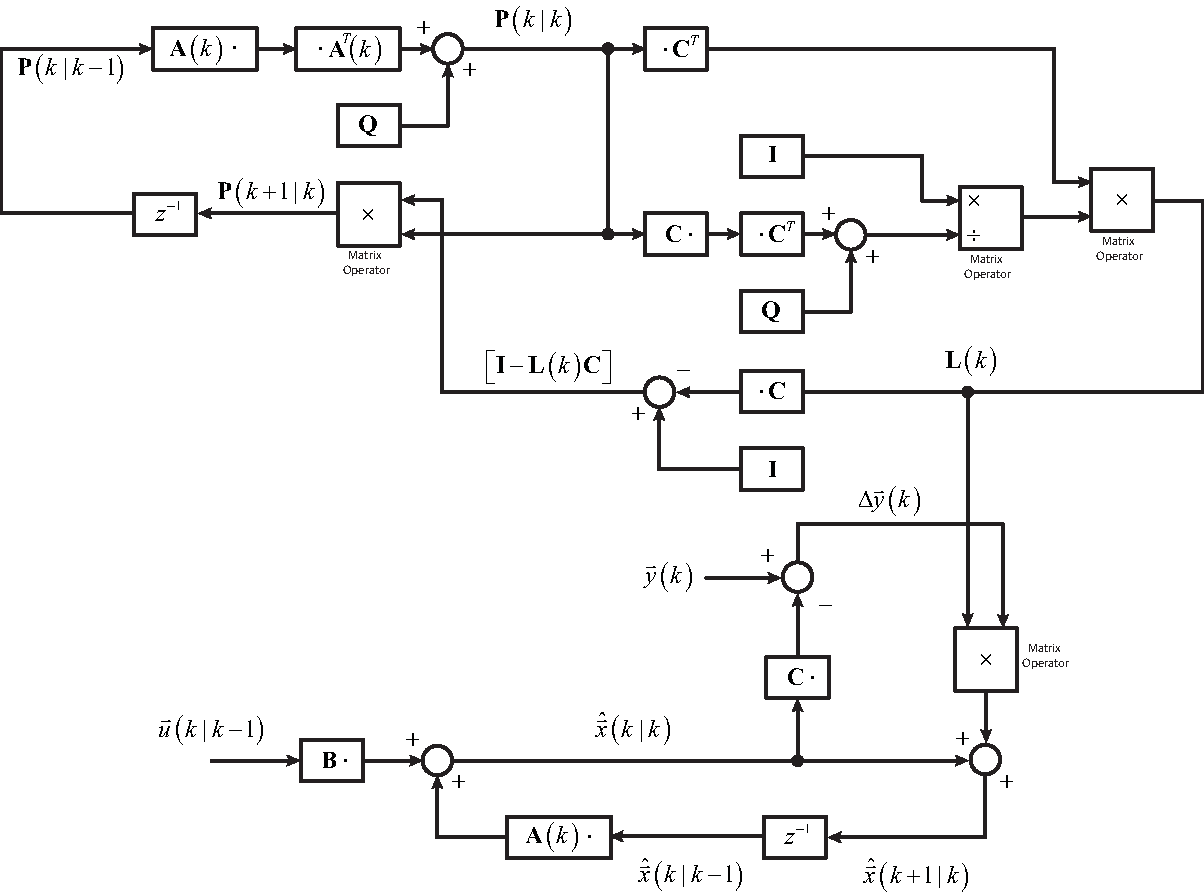
\includegraphics[width = 440pt, angle=0, 
		keepaspectratio]{figures/mpc/kalman_3.pdf}
		\captionsetup{width=.5\textwidth}
		\caption{Kalman observer with time varying matrix transition.}
		\label{EKF}
	\end{figure}
\end{mybox}
%\textbf{Discretization.}
%Considering a discretization process at sampling time $t_s$, the equivalent 
%discrete-time model can be approximated as follows:
%\begin{equation}
%	\mathbf{A} = \mathbf{I} + \tilde{\mathbf{A}} \,t_s
%\end{equation}
%\begin{equation}
%	\mathbf{B} = \tilde{\mathbf{B}} \,t_s
%\end{equation}
%\begin{equation*}\label{twophase_ss1d}
%	\left\lbrace \begin{aligned}
	%		{\vec{x}}(k+1) &= {\mathbf{A}}\,\vec{x}(k) + 
	%{\mathbf{B}}\,\vec{u}_{\alpha\beta}(k) \qquad \vec{x}(0) = \begin{bmatrix} 
		%0 & 0 & \Psi^M &  0 \end{bmatrix}^T\\[6pt]
	%		{\vec{y}}(k) &= {\mathbf{C}}\,\vec{x}(k)
	%	\end{aligned}\right. 
%\end{equation*}

\subsection{EKF Observer for nonlinear PMSM}
In additional to the previous EKF observer, we consider now the case where the torque expression is taken into account into the linearization along the observed state trajectory.
\begin{align}\label{}
	\frac{d}{dt}\vec{x}(t)=\vec{g}(\vec{x})\Rightarrow\left\lbrace 
	\begin{aligned}
		\begin{split}
			&\frac{d}{dt}i_\alpha(t) = -\frac{R_s}{L_s}i_\alpha(t) + 	
			\frac{1}{L_s}\omega(t)\psi_\beta^r(t) + \frac{1}{L_s} u_\alpha(t) 
		\end{split}	\\[6pt]
		\begin{split}
			&\frac{d}{dt}i_\beta(t) = -\frac{R_s}{L_s}i_\beta(t) - 	
			\frac{1}{L_s}\omega(t)\psi_\alpha^r(t) + \frac{1}{L_s} u_\beta(t)	
		\end{split}	\\[6pt]
		\begin{split}
			&\frac{d}{dt}\psi_\alpha^r(t) = -\omega(t)\psi_\beta^r(t)
		\end{split}	\\[6pt]
		\begin{split}	
			&\frac{d}{dt}\psi_\beta^r(t) = \omega(t)\psi_\alpha^r(t)	
		\end{split}	\\[6pt]
		\begin{split}
			&\frac{d}{dt}\vartheta(t) = \omega(t)
		\end{split}	\\[6pt]
		\begin{split}
			&\frac{d}{dt}\omega(t) = 
			\frac{p}{J}\Bigg\{\frac{3}{2}p\Big[\psi^r_{\alpha}(t)i_{\beta}(t) - 
			\psi^r_{\beta}(t)i_{\alpha}(t)\Big] - \tau_l(t) 
			-\frac{b}{p}\omega(t)\Bigg\}
		\end{split}
	\end{aligned}\right. 
\end{align}
where we assumed $L_\alpha = \L_\beta = L_s$ and $\frac{1}{p}\omega(t) = \omega_m(t)$.
\begin{mybox}
	\begin{equation}\label{}
		\begin{aligned}
			\left.\frac{\partial}{\partial 
				\vec{x}}\vec{g}(\vec{x})\right|_{\vec{x}=\hat{\vec{x}}} &= 
			\begin{bmatrix} \frac{\partial g_1}{\partial x_1} & \cdots & 
				\frac{\partial g_1}{\partial x_n} \\[6pt]
				\vdots & \ddots & \vdots \\[6pt]
				\frac{\partial g_n}{\partial x_1} & \cdots & \frac{\partial 
					g_n}{\partial x_n}
			\end{bmatrix}_{\hat{\vec{x}}(t)} \\[8pt]
			&= \begin{bmatrix} 
				-\frac{R_s}{L_s} & 0 & 0 & \frac{\hat{\omega}}{L_s} & 0 & \frac{\hat{\psi}_\beta}{L_s} \\[6pt]			
				0 & -\frac{R_s}{L_s} & -\frac{\hat{\omega}}{L_s} & 0 & 0 & -\frac{\hat{\psi}_\alpha}{L_s} \\[6pt]
				0 & 0 & 0 & -\hat{\omega} & 0 & -\hat{\psi}_\beta \\[6pt]
				0 & 0 & \hat{\omega} & 0 & 0 & \hat{\psi}_\alpha \\[6pt]
				0 & 0 & 0 & 0 & 0 & 1 \\[6pt]
				-\frac{3}{2}\frac{p^2}{J}\hat{\psi}_\beta & \frac{3}{2}\frac{p^2}{J}\hat{\psi}_\alpha
				& \frac{3}{2}\frac{p^2}{J}\hat{i}_\beta & -\frac{3}{2}\frac{p^2}{J}\hat{i}_\alpha & 0 & -\frac{b}{J}
			\end{bmatrix}  \\[8pt]
			&=\tilde{\mathbf{A}}_1 + 
			\hat{\omega}(t) \tilde{\mathbf{A}}_2 + \hat{\psi}_\alpha^r(t) 
			\tilde{\mathbf{A}}_3 + \hat{\psi}_\beta^r(t) \tilde{\mathbf{A}}_4
			+ \hat{i}_\alpha(t) 
			\tilde{\mathbf{A}}_5 + \hat{i}_\beta(t) \tilde{\mathbf{A}}_6
		\end{aligned}
	\end{equation} 
	where $\hat{\vec{x}}$ is the estimated state vector from the EKF.
\end{mybox}

The matrices $\tilde{\mathbf{A}}_1$, $\tilde{\mathbf{A}}_2$, 
$\tilde{\mathbf{A}}_3$, $\tilde{\mathbf{A}}_4$, $\tilde{\mathbf{A}}_5$ and $\tilde{\mathbf{A}}_6$ are as follows
\begin{equation}\label{}
	\begin{aligned}
		&\tilde{\mathbf{A}}_1 = 
		\begin{bmatrix} 
			-\frac{R_s}{L_s} & 0 & 0 & 0 & 0 & 0 \\[6pt]			
			0 & -\frac{R_s}{L_s} & 0 & 0 & 0 & 0 \\[6pt]
			0 & 0 & 0 & 0 & 0 & 0 \\[6pt]
			0 & 0 & 0 & 0 & 0 & 0 \\[6pt]
			0 & 0 & 0 & 0 & 0 & 1 \\[6pt]
			0 & 0 & 0 & 0 & 0 & -\frac{b}{J}
		\end{bmatrix},\quad
		\tilde{\mathbf{A}}_2 = 
		\begin{bmatrix} 
			0 & 0 & 0 & \frac{1}{L_s} & 0 & 0 \\[6pt]			
			0 & 0 & -\frac{1}{L_s} & 0 & 0 & 0 \\[6pt]
			0 & 0 & 0 & -1 & 0 & 0 \\[6pt]
			0 & 0 & 1 & 0 & 0 & 0 \\[6pt]
			0 & 0 & 0 & 0 & 0 & 0 \\[6pt]
			0 & 0 & 0 & 0 & 0 & 0
		\end{bmatrix} \\[8pt]
	\end{aligned}
\end{equation}

\begin{equation}
	\begin{aligned}
		&\tilde{\mathbf{A}}_3 = 
		\begin{bmatrix} 
			0 & 0 & 0 & 0 & 0 & 0 \\[6pt]			
			0 & 0 & 0 & 0 & 0 & -\frac{1}{L_s} \\[6pt]
			0 & 0 & 0 & 0 & 0 & 0 \\[6pt]
			0 & 0 & 0 & 0 & 0 & 1 \\[6pt]
			0 & 0 & 0 & 0 & 0 & 0 \\[6pt]
			0 & \frac{3}{2}\frac{p^2}{J} & 0 & 0 & 0 & 0
		\end{bmatrix},\quad
		\tilde{\mathbf{A}}_4 = 
		\begin{bmatrix} 
			0 & 0 & 0 & 0 & 0 & \frac{1}{L_s} \\[6pt]			
			0 & 0 & 0 & 0 & 0 & 0 \\[6pt]
			0 & 0 & 0 & 0 & 0 & -1 \\[6pt]
			0 & 0 & 0 & 0 & 0 & 0 \\[6pt]
			0 & 0 & 0 & 0 & 0 & 0 \\[6pt]
			-\frac{3}{2}\frac{p^2}{J} & 0 & 0 & 0 & 0 & 0
		\end{bmatrix} 
	\end{aligned}
\end{equation} 

\begin{equation}
	\begin{aligned}
		&\tilde{\mathbf{A}}_5 = 
		\begin{bmatrix} 
			0 & 0 & 0 & 0 & 0 & 0 \\[6pt]			
			0 & 0 & 0 & 0 & 0 & 0 \\[6pt]
			0 & 0 & 0 & 0 & 0 & 0 \\[6pt]
			0 & 0 & 0 & 0 & 0 & 0 \\[6pt]
			0 & 0 & 0 & 0 & 0 & 0 \\[6pt]
			0 & 0 & 0 & -\frac{3}{2}\frac{p^2}{J} & 0 & 0
		\end{bmatrix},\quad
		\tilde{\mathbf{A}}_6 = 
		\begin{bmatrix} 
			0 & 0 & 0 & 0 & 0 & 0 \\[6pt]			
			0 & 0 & 0 & 0 & 0 & 0 \\[6pt]
			0 & 0 & 0 & 0 & 0 & 0 \\[6pt]
			0 & 0 & 0 & 0 & 0 & 0 \\[6pt]
			0 & 0 & 0 & 0 & 0 & 0 \\[6pt]
			0 & 0 & \frac{3}{2}\frac{p^2}{J} & 0 & 0 & 0
		\end{bmatrix} 
	\end{aligned}
\end{equation} 
The discretization of the transition matrix $\tilde{\mathbf{A}}(t)$ can be 
approximated by Taylor as follows
\begin{equation}\label{}
	\begin{aligned}
		{\mathbf{A}}(k|k-1) &= \mathbf{I}_6 + \tilde{\mathbf{A}}_1t_s + 
		\hat{\omega}(k|k-1) \tilde{\mathbf{A}}_2t_s +\\[8pt]
		&\quad + \hat{\psi}_\alpha^r(k|k-1) \tilde{\mathbf{A}}_3t_s  + \hat{\psi}_\beta^r(k|k-1) \tilde{\mathbf{A}}_4t_s +\\[8pt]
		&\quad + \hat{i}_\alpha(k|k-1) \tilde{\mathbf{A}}_5t_s + \hat{i}_\beta(k|k-1) \tilde{\mathbf{A}}_6t_s.
	\end{aligned}
\end{equation}

\end{onehalfspace}
\end{document} 